\documentclass[11pt]{article}

%% Language and font encodings
\usepackage[english]{babel}
\usepackage[utf8x]{inputenc}
\usepackage[T1]{fontenc}
\usepackage[section]{placeins}
\usepackage{graphicx}
\usepackage{caption}
\usepackage{subcaption}
\usepackage{float}
\usepackage{verbatim}
\usepackage{color,soul}
\usepackage{indentfirst}
\usepackage{listings}
\usepackage{fancyhdr}
\usepackage{sectsty}
\sectionfont{\centering}
\usepackage{abstract}
\usepackage{vhistory}
\renewcommand{\abstractnamefont}{\normalfont\Large\bfseries}
%% Sets page size and margins
\usepackage[a4paper,top=3cm,bottom=1cm,left=1cm,right=1cm]{geometry}

%% Useful packages
\usepackage{amsmath}
\usepackage[colorinlistoftodos]{todonotes}
\usepackage[colorlinks=true, allcolors=blue]{hyperref}
\usepackage{listings}
\usepackage{color} %red, green, blue, yellow, cyan, magenta, black, white
\definecolor{mygreen}{RGB}{28,172,0} % color values Red, Green, Blue
\definecolor{mylilas}{RGB}{170,55,241}
\setlength{\parindent}{2em}
\setlength{\parskip}{.75em}

\date{\today}

\begin{document}


\begin{titlepage}
	\centering
    \begin{minipage}{0.05\textwidth}


    \end{minipage}
    \rule[-400pt]{1.5pt}{600pt}
    \hspace*{0.05\textwidth} % Whitespace between the vertical line and title page text
    \begin{minipage}{0.5\textwidth}
        
\includegraphics[width=\textwidth]{osu.jpg}\par\vspace{1cm}
        \vspace{.5cm}
    	{\scshape\Large ECE 44x - Group 3  \par Automated Microbial Analysis\par}
    	\vspace{1cm}
    	{\huge\bfseries Reading and Implications Report \par}
    	{\large\bfseries Mechanical Design - Connectors and Enclosures \par}
    	\vspace{1cm}
    	{\Large\itshape Jorian Bruslind\par}

	    \vspace{1cm}
    \vspace{.25cm}
    \end{minipage}


% Bottom of the page
	{\large \today\par}
\end{titlepage}
\newgeometry{top=2.5cm,bottom=2.5cm,right=2cm,left=2cm}
\tableofcontents

\newpage


\pagestyle{fancy}
\fancyhf{}
\rhead{Automated Microbial Analysis}
\lhead{Mechanical Design}
\rfoot{Page \thepage}

\begin{abstract}
    The purpose of this document is to provide context for the reader behind the design choices made within the perview of the mechanical design aspect of the Automated Microbial Analysis capstone project. This project aims to manipulate, analyze, and physically sort microbial samples present on 3M Petrifilm. This document will cover the mechanical concepts present in the system, the design choices for each concept and the proposed solution for each choice. Finally, this document will then cover the expected challenges with this project and possible solutions to said challenges. 
\end{abstract}

\section{Introduction}

The Automated Microbial Analysis project aims to develop a system which is able to analyze a series of microbial samples on a special media called PetriFilm \cite{beveragedaily.com2014May} automatically. This is a 3M product that is used in a variety of scientific capacities, mainly in food science and the medical field. 

\begin{figure}[H]
    \centering
    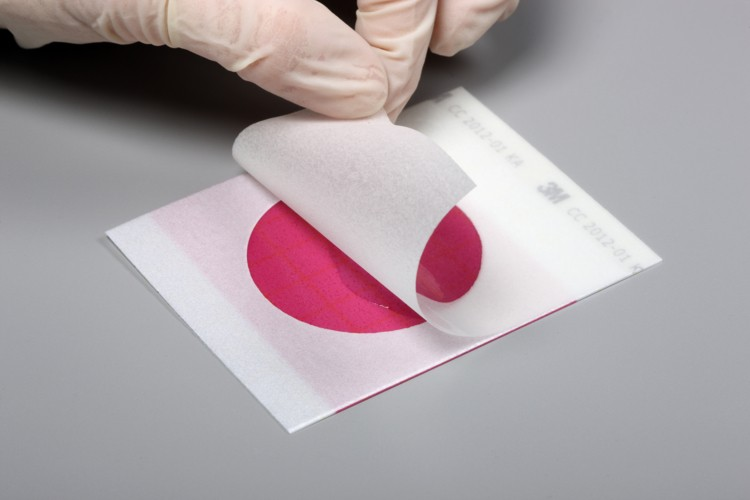
\includegraphics[width = .5\textwidth]{Pictures/3MPetrifilm.jpg}
    \caption{3M PetriFilm Single Sample}
    \label{fig:Petrifilm}
\end{figure}



PetriFilm is a very thin paper-like substance which has 2 layers: on one there is an agar media film that is used to grow bacterium, On the other there is a wax coating that is used to seal the sample from outside interference. A liquid sample can be applied to this agar film and left to incubate over a period of 1 - 2 days. After this time, the bacteria that were present within the sample will have  had enough time to grow into colonies which are visible to the human eye. These colonies can be counted and the original number of bacterium per unit volume can be known from the original sample. The process to count the bacteria samples and categorize them into datasets is often tedious and can take a human operator around 1 - 2 minutes per sample \cite{3M_Interpretation}. With sample sizes of 50 - 60, this process can easily take over an hour. The goal of our project is to use an automated system to count these bacteria colonies in sample sets of upwards of 100+ in as little as 20 minutes. This data will be automatically stored and tabulated within the client's original database. 



For this process it is necessary to create a physical manipulation system that will be able to move paper-like objects in an efficient and precise manner. These samples are somewhat delicate and require careful handling. In addition, they must be placed in a specific orientation so that the bacterial samples can be easily read by some visual component. Therefore it is necessary to create a mechanical system that can be easily made precise and is able to be used for our intended implementation. In addition, there will be designated areas for loading/unloading of samples so that the overall process requires as little human intervention as possible.  



Once the loaded, the system will take over and begin the counting process for each sample. There will be error correction and state information for each portion of the counting cycle to ensure the samples are not damaged and to reduce the chance of a miscount. After the sample has been counted and cataloged, it will be placed into one of two sections designated "Pass" or "Needs Review" where they can be sorted by a human operator. 



This document aims to provide context for my responsibilities as they apply to the project and what steps were taken to achieve the goals outlined above. I have personally been involved in a variety of robotics related projects working with groups ranging from 1 - 20 people. I have had experience working with control systems, mechanical design, and automated systems and it is my hope that I can apply that experience towards the success of this project. 

\section{Summary of Expert Topic Areas and Design Challenges}

This project requires a great deal of mechanical, electrical and computer science engineering and necessitates the complexity of having each area work together. To help simplify the design process, each team member is assigned an area of expertise that they are responsible for. For me specifically, I will be responsible for the mechanical design and hardware implementation of our system. 

\subsection{Area of Expertise}

For this project, 2 mechanical systems came to mind that are used in similar applications. The first being a printer while the second was a pick and place machine. Both use fairly intricate mechanical systems to preform their function and as such I need to be aware of their abilities and limitations. It is important to consider parameters such as speed, simplicity in design, cost, and ease of use when designing a system such as ours and it will be my responsibility to analyze each when considering the different options. 

For this area of expertise, I will need to be responsible for the design and simulation of our mechanical system. To do so I will use Computer Assisted Design (CAD) in the form of Autodesk Inventor to model our entire system before assembly. I have had around 6 years experience working with Inventor in other applications and feel confident in it's ability for CAD modeling. 

\subsection{Design Challenges}

The project requirements that most relate to my area of expertise include: Accuracy, Sample Preservation, Fast, Enclosed Work Area, and Ease of Use. All of these requirements require the mechanical system in some way, shape or form. With this in mind my research focused on the possible mechanical systems and their ability to meet the aforementioned requirements. Speed and accuracy were the two requirements I spend the most amount of focus on as they were ultimately the most influential in deciding which mechanism to go with. In addition, most all systems can be designed in such a way to be easy to use, have an enclosed work area, and prioritizing accuracy provides a means for sample preservation. 

A focus of my research was what mechanical systems were used in industry for similar purposes to ours. The point being that many companies would have invested time and money into figuring out the most efficient way to preform their specific task. First, an analysis of the task that is to be preformed indicated 2 possible mechanisms: Pick and Placing and printing/scanning. The PetriFilm can be thought of as slips of paper in the fact that they are both light and thin. Therefore, the most common forms of industrial robotics that deal with paper-like objects are through printing/scanning mechanisms and pick/placing mechanisms \cite{robot_types}. The printing/scanning methods (as seen in \ref{fig:printer})seem to be the most ideal, considering the act of imaging paper is the same process that we must do to the PetriFilm. Within the pick and placing category, the most popular type of robots found in industry include the Delta robot configuration \ref{fig:Delta} and the Cartesian (Gantry) robot configuration \ref{fig:Gantry}. For simplicity, I will focus on the contrasts between our 3 stated requirements and the aforementioned robotic systems. 


    \begin{figure}[H]
    \centering
    \begin{subfigure}{.3\textwidth}
      \centering
      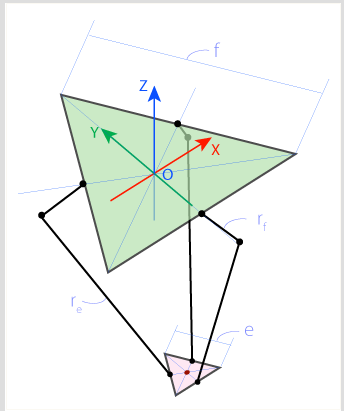
\includegraphics[width=.7\linewidth]{Delta_arms.png}
      \caption{Modeled Delta Robot)}
      \label{fig:Delta}
    \end{subfigure}%
    \begin{subfigure}{.3\textwidth}
      \centering
      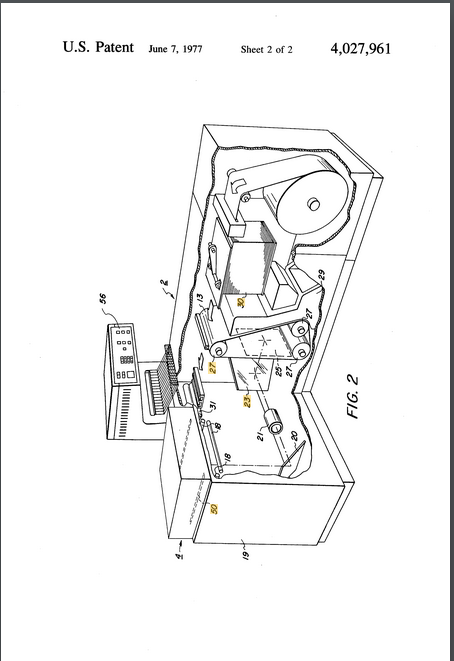
\includegraphics[width=.7\linewidth]{Printer_Schematic.png}
      \caption{Simple Printer Schematic)}
      \label{fig:printer}
    \end{subfigure}
    \label{fig:test}
    \begin{subfigure}{.3\textwidth}
      \centering
      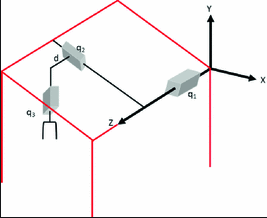
\includegraphics[width=.7\linewidth]{Gantry_Kinematics.png}
      \caption{Modeled Gantry Robot}
      \label{fig:Gantry}
    \end{subfigure}
    \label{fig:test}
    \end{figure}


%Links
%https://www.researchgate.net/publication/319876160_Mechanical_Design_of_a_Cartesian_Manipulator_for_Warehouse_Pick_and_Place - Delta Speed
%https://patents.google.com/patent/US4027961 - complex printer
%http://cms.gcg11.ac.in/attachments/article/102/Printers,types%20,working%20and%20use..pdf - Slides about printers
%https://www.plantautomation-technology.com/articles/types-of-robots-based-on-configuration - compare/contrast robots

\section{Challenge 1 - Accuracy}

Arguably, the most important aspect of our project is that is must be accurate so as not to damage the provided samples and to improve it's overall time cost for this process (less mistakes mean less time needed to recover). To measure accuracy, I investigated 2 components of the mechanical systems, the end effector accuracy and what steps are necessary to improve the end effector accuracy. The end effector in this case is whatever part is going to be moving the samples during the process. It is necessary to also investigate possible improvements to the accuracy of the systems as some systems may not have the best inherent stability, but for relatively little cost they could be improved. For simplicity, I am assuming all motors used are NEMA 17 200 step/rev 2 phase stepper motors \cite{Nema17} so as to standardize the investigation. 

\begin{figure}[H]
    \centering
    \begin{subfigure}{.4\textwidth}
        \centering
        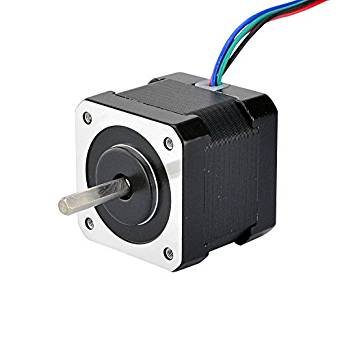
\includegraphics[width = .7\textwidth]{NEMA17.jpg}
        \caption{NEMA 17 Stepper Motor}
        \label{fig:NEMA17Step}
    \end{subfigure}
    \begin{subfigure}{.4\textwidth}
        \centering
        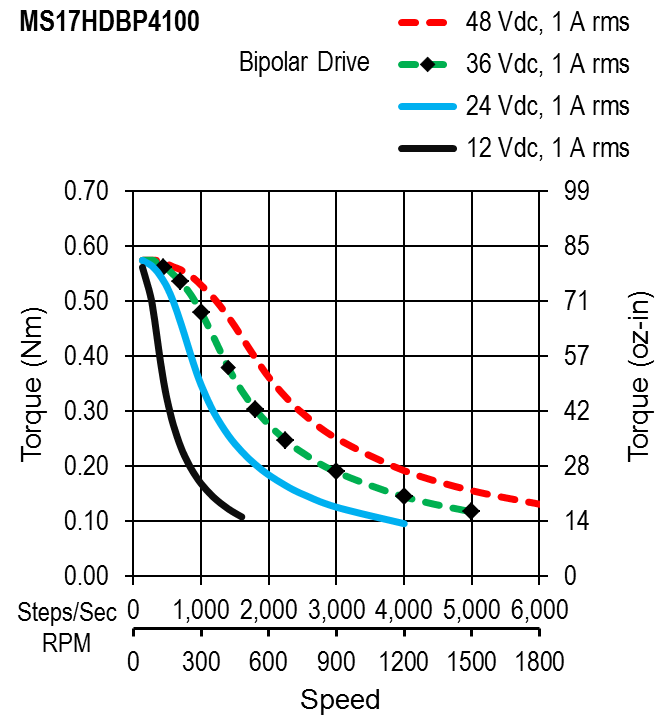
\includegraphics[width = .7\textwidth]{Torque_NEMA17.png}
        \caption{NEMA 17 Torque Curve \cite{NEMATorque}}
        \label{fig:NEMA17torque}
    \end{subfigure}
\end{figure}

If we were to model our design after a printer/scanner then it would be accurate to within a few mm, however it comes at the cost of many different sensors and a complex mechanical system. Looking at the overall design of a printer system, it can be seen that in order to facilitate the processing of samples in a stack, there must be mechanisms that keep the stack in order, in place, and restricted enough so that only 1 sample is taken at one time. It is known that printers will often experience jams or other physical problems that would ultimately destroy the samples if they occurred. So while it may be possible to achieve accuracy to a fine degree, the amount of extra work required to achieve this is beyond the scope of our ability. 

%https://mindmachine.co.uk/book/print_18_paperfeed.html

Other possible options for this design would be to employ a robotic system to manipulate samples within a set workspace. Both Gantry and Delta robots are renown for their ability or preform pick and place operations accurately. The reason for choosing pick and place for our operation is that samples can easily be put into a stack and picked off / placed down for analysis. 

Of the two options, the easiest to understand is probably the Cartesian (Gantry) robot. This mechanical system is simple in that it just uses 1 stepper to move in each Cartesian direction. Therefore the accuracy of the overall system is just limited by the accuracy of the chosen stepper motor. Depending on the operation, it may be necessary to scale the torque of the stepper motor through gear/pulley ratios which would ultimately reduce the overall accuracy \cite{Stepper_Pulley}, but for the purposes of this document we will assume there is no reduction. 

    \begin{figure}[H]
        \centering
        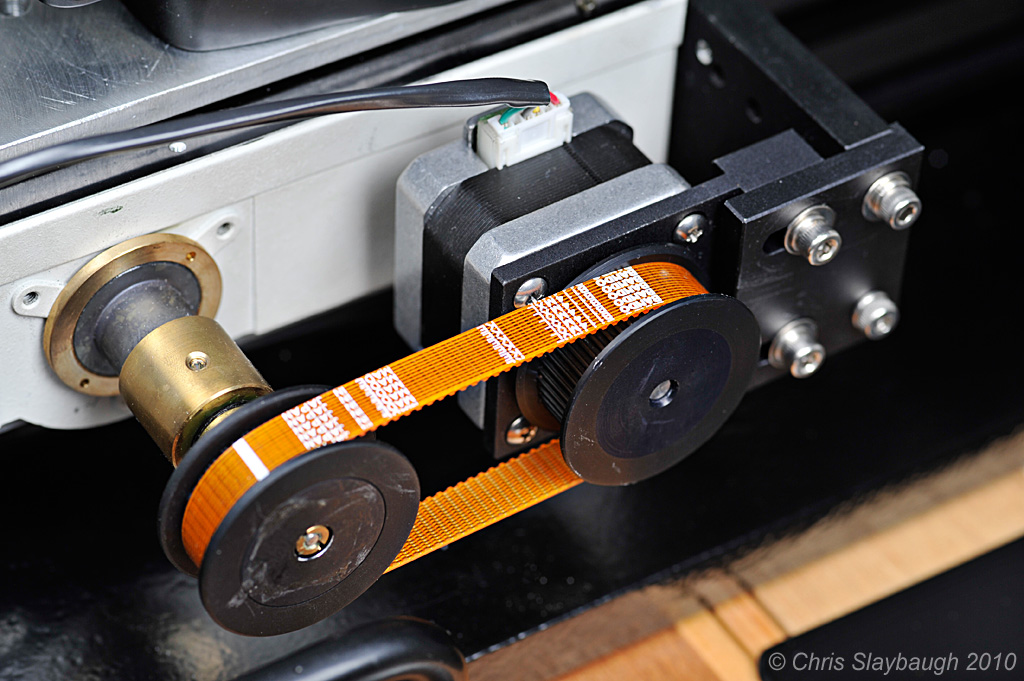
\includegraphics[width = .5\textwidth]{Stepper_pulley.jpg}
        \caption{Possible gear reduction using pulley}
        \label{fig:forward_kin}
    \end{figure}

The Delta robot is a little more complicated in the analysis of accuracy. Similar to the Gantry robot, the accuracy is directly related to the chosen stepper motors, however the error factor is multiplied by a factor related to the delta robot armature length. This is due in fact to the idea that the stepper will drive a longer arm which in turns moves the end effector. Therefore a small error on part of the rotation of the stepper, will induce a larger error (translationally) at the end of the arm length (arc length vs angle). Therefore the Delta robot will have a similar accuracy to the Gantry robot just scaled by a factor of the chosen armature length. 


    \begin{figure}[H]
    \centering
    \begin{subfigure}{.5\textwidth}
      \centering
      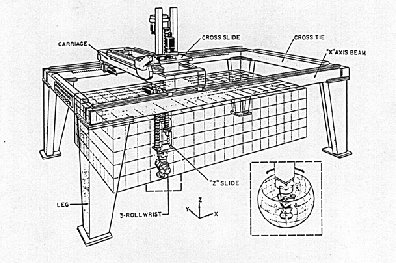
\includegraphics[width=.7\linewidth]{gantry_workarea.jpg}
      \caption{Gantry work area}
      \label{fig:Gantry_Work}
    \end{subfigure}%
    \begin{subfigure}{.5\textwidth}
      \centering
      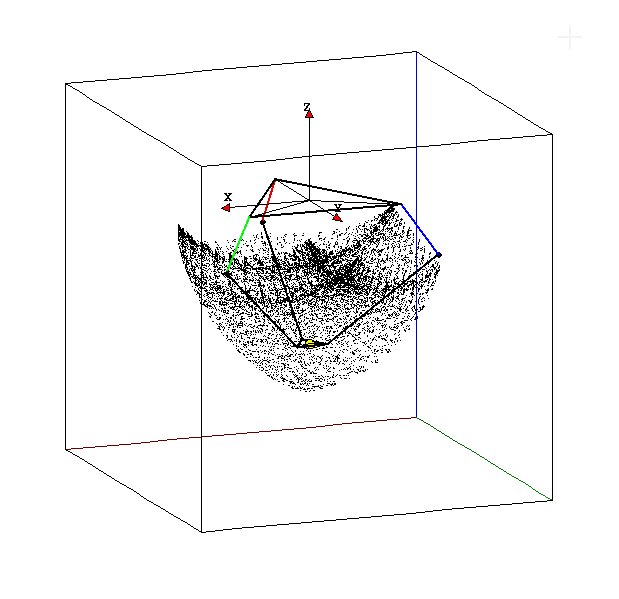
\includegraphics[width=.7\linewidth]{Delta_Workarea.png}
      \caption{Delta work area from simulation \cite{Delta_Sim}}
      \label{fig:Delta_Work}
    \end{subfigure}
    \label{fig:test}
    \end{figure}

\section{Challenge 2 - Speed}

Speed is also an important consideration for this project. while accuracy ensures the samples will not be damaged, speed is ultimately speed is why the project exists at all. In order to consider the project effective, it must be able to move samples on the order of 100 / 5 - 10 min. With this in mind, I thought of speed as very close (but not quite as) important as accuracy.  

For the Gantry robot, speed is limited to the abilities of the chosen stepper motors and the location of the sample input/output stacks \cite{Cartisian_Design}. This can be amplified through the use of gearboxes or pulley systems, with the cost of losing some torque or overall force power. 

The Delta robot is a little more complicated. The speed that this mechanism can achieve is mostly based off of its armature length as explained above. For every $1^\circ$ of rotation, the actual movement is based off the arc length which is in turn based off the length of the armature. By deriving the Delta robot's forward kinematic equations (where, given ($\Theta_1, \Theta_2, \Theta_3$) we can determine ($X_0, Y_0, Z_0$)), it is possible to determine by what factor the actual speed is increased. Using the model variables found in \ref{fig:Delta_Label} the derivation follows between images \cite{TrossenRobotics}.

    \begin{figure}[H]
    \centering
    \begin{subfigure}{.5\textwidth}
      \centering
      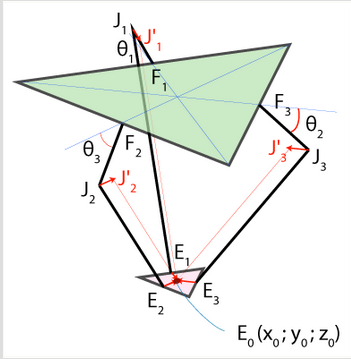
\includegraphics[width=.7\linewidth]{Delta_Labeld.png}
      \caption{Labeled Delta Variables}
      \label{fig:Delta_Label}
    \end{subfigure}%
    \begin{subfigure}{.5\textwidth}
      \centering
      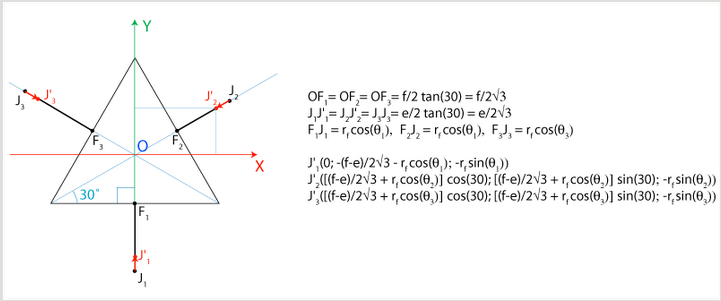
\includegraphics[width=.7\linewidth]{Delta_math_fig.png}
      \caption{Defining Delta parameters with corresponding equations}
      \label{fig:Delta_math_fig}
    \end{subfigure}
    \label{fig:test}
    \end{figure}
    
    \begin{figure}[H]
        \centering
        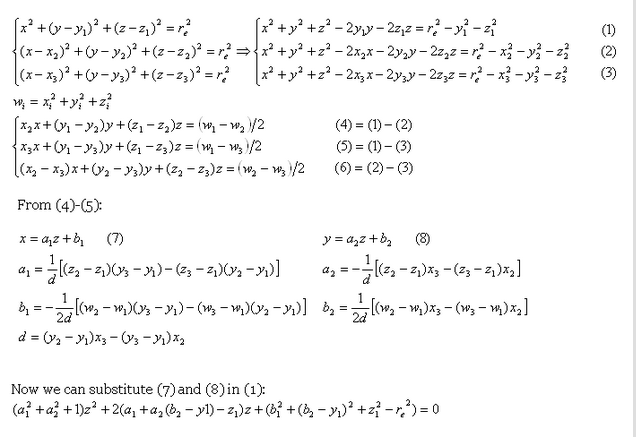
\includegraphics[width = .5\textwidth]{Delta_Math.png}
        \caption{Forward Kinematics calculations}
        \label{fig:forward_kin}
    \end{figure}
    
Generalizing from \ref{fig:forward_kin} we can determine that the rotation of all 3 motors $1^\circ$ would increase the Z axis parameter by a factor of $cos(\theta) \cdot F_x$ where $F_x$ is the given armature length. 

\section{Challenge 3 - Ease of Use}

While it may be possible to achieve a mechanism that is fast and accurate, it must also be easy to use. For this we are defining "easy to use" as a mechanism that can be assembled with few unique parts, has a wide range of support online/offline and requires few fastener components. Seeing as we cannot model and simulate both mechanism, I will analyze using the available data from similar designs built online.  

The Gantry robot is easy to understand and thus has an overall advantage in this area. Using the RepRap Hydra prototype \ref{fig:Hail_Hydra} Gantry robot we can see that overall it is not a terribly complex design with few fasteners and necessary mounting points \cite{Gantry_Exploded}.  This would make the gantry and ideal candidate for an easy to use system. In addition, since the increase in 3D printing technology, there is a wide range of online support through forums and manuals that will allow for inspiration in the design/build process. 

    \begin{figure}[H]
        \centering
        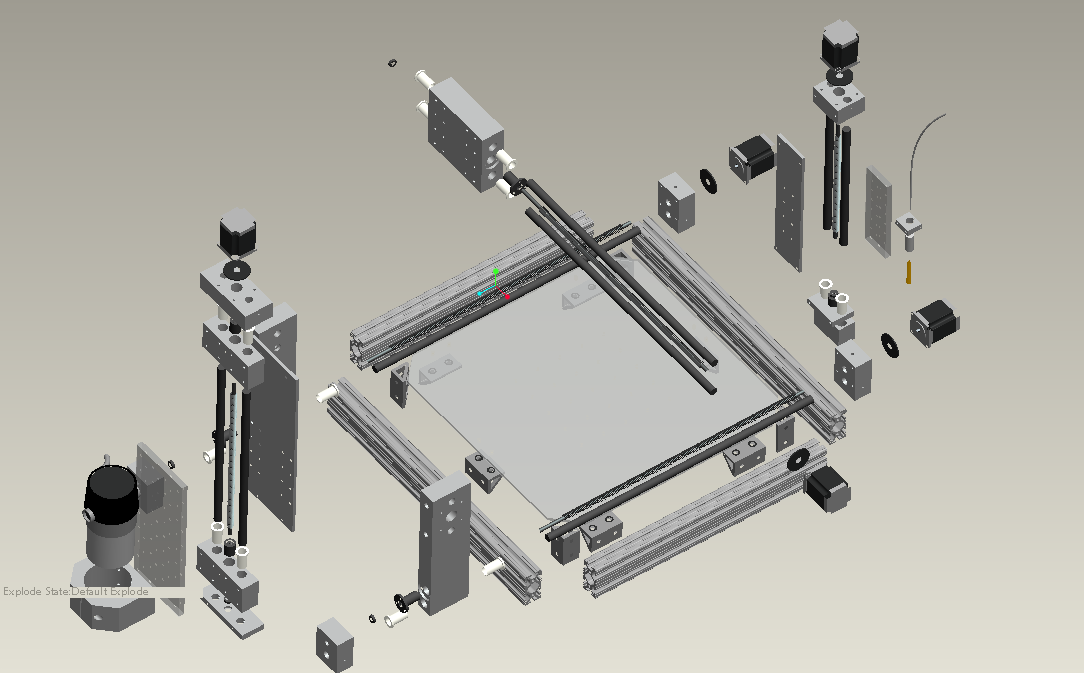
\includegraphics[width = .5\textwidth]{Hydra_Exploded_view2.png}
        \caption{Hydra Gantry Prototype}
        \label{fig:Hail_Hydra}
    \end{figure}
    
The Delta robot has less available online material for possible building structures, save for a few online forums. Based on a custom design it can be seen that the Delta involves a higher level of complexity to it that the Gantry \ref{fig:Delta_Exploded}.

Something to note is that this exploded view only covers 1/3rd of the actual robot mechanism. This was done intentionally to not crowd out the smaller details/components. 

While the delta robot is seen as more complex than the gantry system, it is worth noting that this complexity diminishes as the design progresses. As the system is fleshed out there are only one-time costs towards overall time usage that are spent in comparison to the Gantry robot. For example, once one arm of the Delta robot is decided and designed, this can be copied to the other 3 arms due to the inherent symmetry of the system. The same goes for any other portions of the design related to the linkage design. So while the complexity is increased for designing a Delta robot, this is offset by the fact that these are one-time costs. 

    \begin{figure}[H]
        \centering
        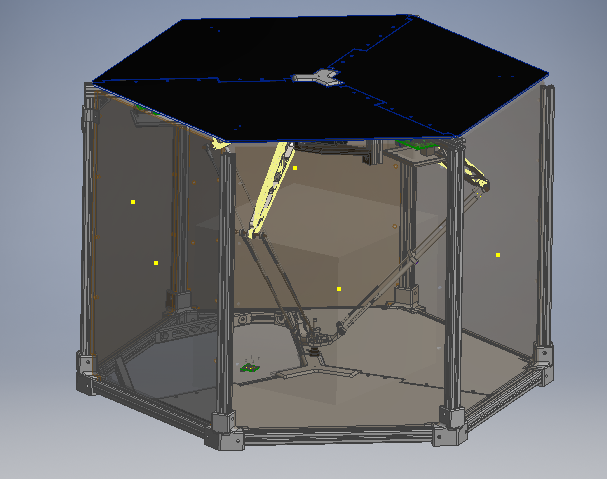
\includegraphics[width = .5\textwidth]{Updated_Assembly_.png}
        \caption{Delta Robot Exploded View}
        \label{fig:Delta_Exploded}
    \end{figure}

\section{Implementation and Discussion}

Being a robotics project there are inherent complexities that must be resolved between subgroups such as the electrical control of the mechanical design, computer commands for electrical control and how effective the mechanical design facilitates the overall process. With that, the project must maintain a high level of communication and simplicity so that all groups are able to understand how their design affects the overall system and others designs \cite{undegrad_robots}.  

Since this system is being designed and manufactured from the ground up, there is the inherent risk that whatever is designed may not work. Working on such a short timeline also means that there will be little time to revise or otherwise improve errors during the build/test phase. This relates back to the complexity component of the chosen mechanical design in which whatever design is chosen must be able to be easily changed or otherwise modified to suit any issues that arise during implementation. 

Between the gantry and delta robot styles they both offer strong benefits in either speed or accuracy. The gantry robot can be considered more precise due to the direct drive system of actuation but is limited to the speed of the drive motors. The delta robot amplifies its drive motor speed by a factor of $cos(\theta)*F_x$ but also amplifies the possible error in movement leading it to lack in accuracy. 

The delta robot seems to be a more attractive offer for this specific application due to its very fast speed and industrial support. The accuracy issues are not extreme and can be improved by the addition of motor encoders which will keep track of possible errors in movement to $\pm 1$ step. The complexity of design can also be simplified through careful effort to create symmetry between the leg/arm units. This design style could also lead to a more efficient design solution even compared to the gantry printer. 

Something to keep in mind is that if the Delta robot fails in the early design stages, there are open source models of gantry robots for CNC or 3D printing applications that could be used as an easy replacement. While lacking in specific benefits towards this project, the gantry is a common and easy design that could be replicated in short order. Using this as a backup solution, this project has a set goal that can be achieved within the allocated time frame. 

\begin{versionhistory}
  \vhEntry{1.0}{12.5.2019}{Jorian Bruslind}{created}
  \vhEntry{1.1}{1.20.2019}{Jorian Bruslind}{Updated final assembly description and profile}
  \vhEntry{1.0}{2.4.2019}{Jorian Bruslind}{Optimized wordings and clarified subjects}
\end{versionhistory}

\bibliographystyle{IEEEtran}
\bibliography{sample}

\end{document}
